\subsection{Randomness of Extra-Mileage}
This section is dedicated to a possible different approach to the Extra-Mileage algorithm. 

In the previous section, this algorithm was described starting using the diameter nodes of the input graph. To add some randomness to the algorithm, we chose to implement a multistart approach with the choice of two random nodes as starting nodes, instead of the diameter.

During each run, within a time limit, two random nodes are chosen as starting node, and then the algorithm proceeds as normal. 

We are using the Performance Profile tool to actually assert whether the diameter start of the Farthest Insertion algorithm was better or not than the random start approach. The results can be seen in Figure \ref{fig:extra}, which shows that the classic approach using the diameter as starting nodes performs better overall.

\begin{figure}[!h]
    \centering
    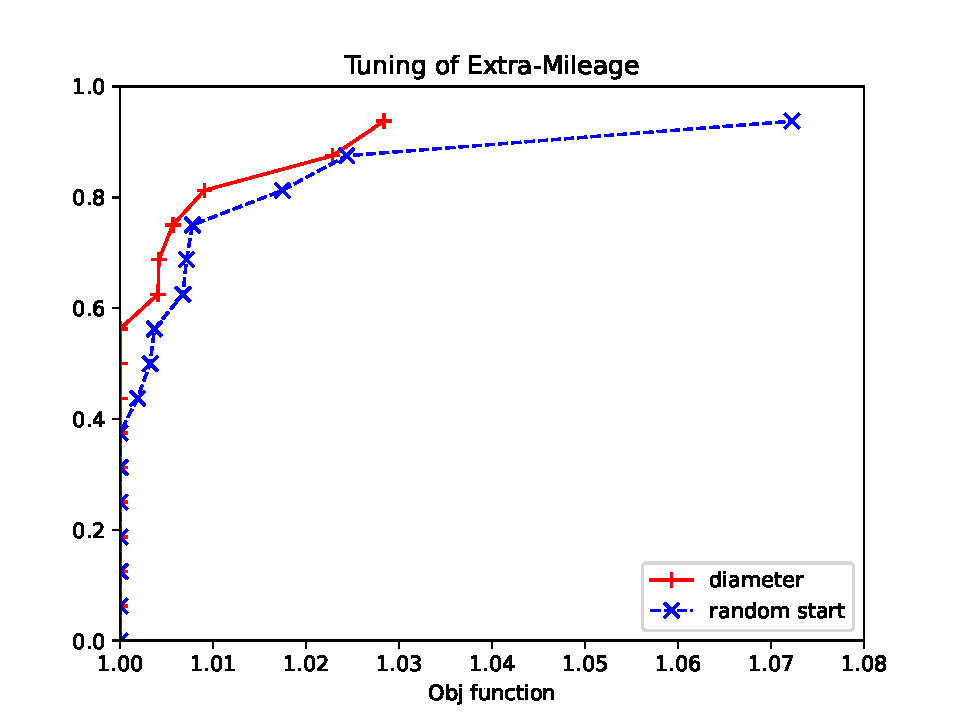
\includegraphics[width=\textwidth]{images/extra.pdf}
    \caption{Tuning of Extra-Mileage}
    \label{fig:extra}
\end{figure}
